\documentclass{beamer}

\usetheme{Warsaw}
\usepackage{graphicx}
% include.tex
\newcommand{\Bernoulli}[1]{\text{Bernoulli} \left( #1 \right)}
\newcommand{\mydigamma}[1]{\psi \left( #1 \right)}
%\newcommand{\diag}[1]{\text{diag}\left( #1 \right)}
\newcommand{\tr}[1]{\text{tr}\left( #1 \right)}
\newcommand{\Poisson}[1]{\text{Poisson} \left( #1 \right)}
\def \half {\frac{1}{2}}
\def \R {\mathbb{R}}
\def \vbeta {\vec{\beta}}
\def \vy {\vec{y}}
\def \vmu {\vec{\mu}}
\def \vmuqbeta {\vmu_{q(\vbeta)}}
\def \vmubeta {\vmu_{\vbeta}}
\def \Sigmaqbeta {\Sigma_{q(\vbeta)}}
\def \Sigmabeta {\Sigma_{\vbeta}}
\def \va {\vec{a}}
\def \vtheta {\vec{\theta}}
\def \mX {\vec{X}}

\def\ds{{\displaystyle}}

\def\diag{{\mbox{diag}}}


\usefonttheme{serif}

\title{Variational approximations to zero-inflated count models}
\author{Mark Greenaway\\PhD candidate\\markg@maths.usyd.edu.au}

\mode<presentation>
{ \usetheme{boxes} }

\begin{document}
% 1. Front slide
\begin{frame}
\titlepage
% Details about myself here?
\end{frame}

% 2. Intro
\begin{frame}
\frametitle{Introduction}
Zero inflated data arises in many areas of application, such as physical
activity data, number of hospital visits and number of insurance claims per
year.

\bigskip 
We will work with zero-inflated count data. I encountered this sort of data while
analysing the data arising from the Get Healthy project.
\end{frame}

% 4. \rho = 9/10, \lambda = 5
% Example data 0 0 0 5 10
\begin{frame}[fragile]
\frametitle{Example data}
\begin{verbatim}
0 7 3 4 5 3 2 6 5 0 0 1
0 0 5 0 2 3 6 4 0 5 4 0
7 0 0 0 7 0 6 6 0 3 0 5
0 4 0 0 0 2 3 0 3 4 5 0
8 0
\end{verbatim}
%Take, for example, $\rho = \frac{1}{2}, \lambda = 5$.

\noindent Note that $n=50$, 
$n\times P(Z = 0) \approx 3.8$ for $Z\sim\mbox{Poisson}(\overline{X})$
and we have observed 21 zeros. Hence,
a Poisson model is not suitable.

% Histogram
% 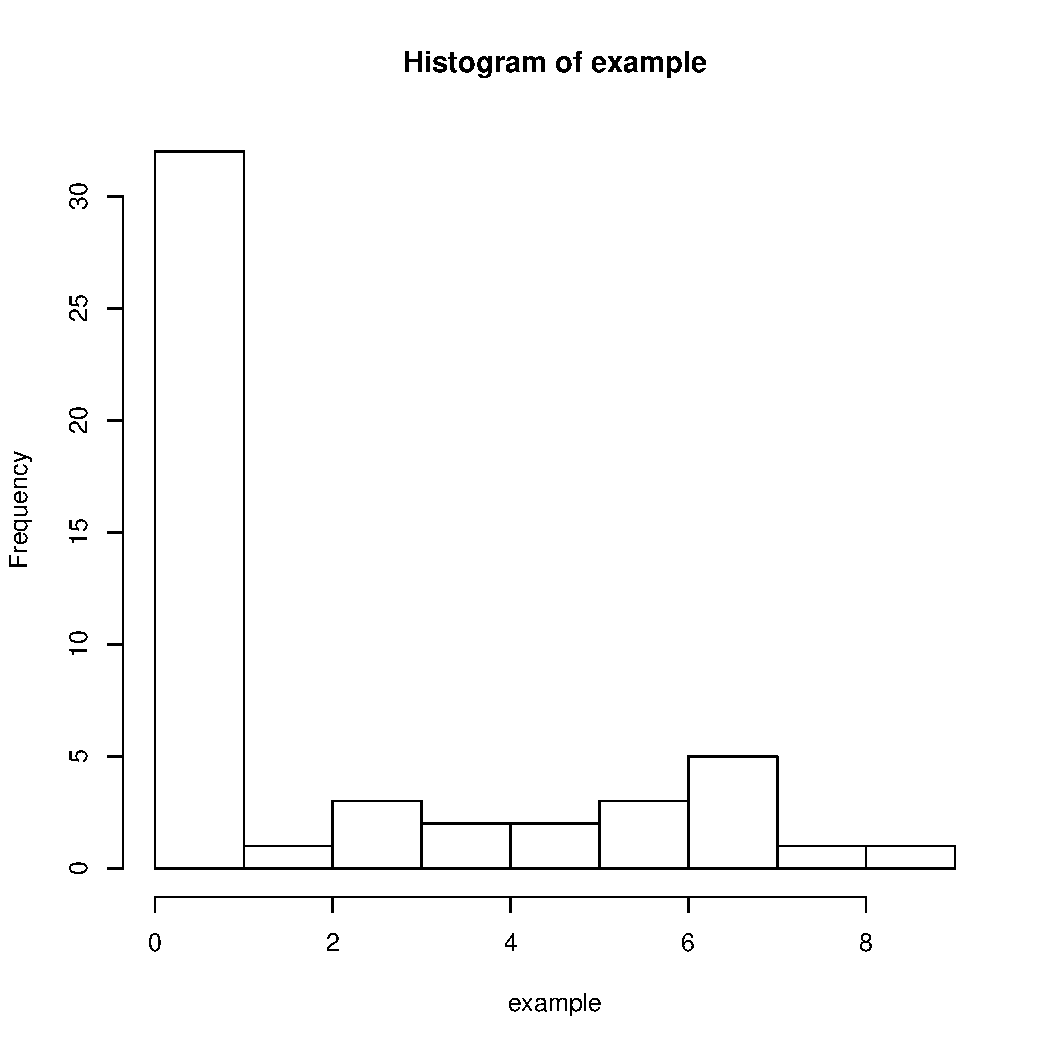
\includegraphics[width=50mm, height=50mm]{code/univariate_data_histogram.pdf}
% Density
\end{frame}

% 3. Univariate model
\begin{frame}
\frametitle{Univariate model formulation}

We start by building a relatively simple zero-inflated count model. Suppose that we observe
$$
X_i = R_i Y_i, \quad 1\le i\le n,
$$

\noindent where for $1\le i\le n$,
\begin{align*} 
R_i &\sim \text{Bernoulli}(\rho) \\
Y_i &\sim \text{Poisson}(\lambda)
\end{align*}

\noindent for parameters $\rho$ and $\lambda$,
but we do not observe $R_i$ or $Y_i$ themselves.
Being Bayesians we use the priors:
\begin{align*} 
\rho &\sim \text{Beta}(a_\rho, b_\rho) \\
\lambda &\sim \text{Gamma}(a_\lambda, b_\lambda).
\end{align*}

\end{frame}

% 5. How to fit, and advantages and disadvantages of each approach
% - Maximum likelihood
% - MCMC
% - VB

\begin{frame}
\frametitle{Comparison of fitting techniques}
\begin{tabular}{p{2cm}p{3.5cm}p{4.5cm}}
Technique & Pro & Con \\
\hline
MLE & EM could be used to fit these models, with $R_i$ as latent data & Not flexible to complications. \\
& & \\ %Frequentist \\
\hline
MCMC & Bayesian & Slow \\
	& Very accurate &  \\
\hline
Variational Bayes & Bayesian & May lose accuracy, or underestimate variance \\
& Fast  & Solution may be intractable \\ 
& Still quite accurate & \\
\hline
\end{tabular}

\end{frame}

% 6. Overview of Variational Bayes
\begin{frame}
\frametitle{An overview of Variational Bayes}
\begin{itemize}
\item \emph{Idea:} Approximate the full posterior $p(\theta|\vx)$ with a simpler approximation $q(\theta)$.

\item Fit $q(\theta)$ to the data by minimising the KL divergence between $p(\theta|\vx)$ and $q(\theta)$.

\item Theory guarantees that $\log p(x)\ge 
\log \underline{p}(x;q)$ and that 
$$
\log \underline{p}(x;q) = \int q(\vtheta) \left\{ \frac{p(\vy,\vtheta)}{q(\vtheta)} \right\}
$$ 

\noindent will
increase with each iteration.

\item If you use conjugate priors, a factored approximation can be used, and mean field updates can be used on
each parameter in turn until convergence is reached.
\end{itemize}
\end{frame}

\begin{frame}
\frametitle{An overview of Variational Bayes - Continued}
% - Algorithm
We iteratively update the parameters of each approximate distribution
in turn until the lower bound of the approximation converges.

\bigskip 
This could be thought of as a generalisation of Expectation Maximisation, where each parameter is thought of as a latent
variable and estimated according to the expectations of the other parameters.
\end{frame}




% 7a. Variational Bayes solution to ZIP
% - q-densities
\begin{frame}
Choose a factored approximation of the form
$$
q(\theta) = q(\lambda) q(\rho) \prod_{i=1}^n q(r_i)
$$
where
\begin{align*}
q(\lambda) &= \text{Gamma}(\alpha_{q(\lambda)}, \beta_{q(\lambda)}) \\
q(\rho) &= \text{Beta}(\alpha_{q(\rho)}, \beta_{q(\rho)}) \\
q(r_i) &= \text{Bernoulli}(p_i)
\end{align*}

% \begin{align*}
% q(\lambda) = \text{Gamma}(a_{\lambda_*}, b_{\lambda_*}) \\
% q(\rho) = \text{Beta}(a_{q(\rho)}, b_{q(\rho)}) \\
% q(r_i) = \text{Bernoulli}(p_i)
% \end{align*}

% - Algorithm
We iteratively update the parameters of each approximate distribution
in turn until the lower bound of the approximation converges.

\end{frame}
 

% 8. Results
% - Lower bound convergence
% - Accuracies
% 7b. Define accuracy
\begin{frame}
\frametitle{Mean field updates}
As we are using conjugate priors in our model, the mean field updates can be derived.
\begin{align*}
q(\lambda) &= \text{Gamma}(\alpha_{q(\lambda)} = \alpha_\lambda + \vone^T \vx, \beta_{q(\lambda)} = \beta_\lambda + \vone^T\vp) \\
q(\rho) &= \text{Beta}(\alpha_{q(\rho)} = \alpha_\rho + \vone^T\vr, \beta_{q(\rho)} = \beta_\rho + \vone^T(\vone - \vr)) \\
q(r_i) &= \text{Bernoulli}(p_i = \text{expit}(\eta_i))
\end{align*}
where
$$
\eta_i = - \frac{\alpha_{q(\lambda)}}{\beta_{q(\lambda)}} + \Psi(\alpha_{q(\rho)}) - \Psi(\beta_{q(\rho)})
$$

\end{frame}

\begin{frame}
\frametitle{Results/Accuracy}
% Definition of accuracy
Accuracy is defined as 1 minus half the difference in $L_1$ norm between the
true posterior distribution and the approximate posterior distribution of the
variational approximation.

$$
\text{Accuracy} = 1 - \half \|p(\vtheta|\vx) - q(\vtheta)\|_1
$$

This was calculated using the kernel density estimate of the posterior
distribution from MCMC minus the approximating distribution for each parameter of
interest.

\bigskip 
There was excellent accuracy for the univariate approximation, over 99\% in all of the cases that I looked at.
% Graph of lower bound
%\includegraphics{univariate_lower_bound_convergence.pdf}
\end{frame}

% 9. Extension to linear model
% 10. Overview GVA
% 11. Algorithm
% 12. Results?
% 13. What next
% 14. Conclusion
% 15. References
\begin{frame}
\frametitle{Extension to multivariate/regression models}
\begin{itemize}
\item Univariate models are a nice proof of concept.
\item Most applied statisticians want to build regression models.
\item Applied statisticians love mixed models.
\item There is a need for better approaches to fitting zero-inflated mixed models.
\item For example, MCMC with existing software can take minutes to
converge, or not converge at all.
\item That might not sound so bad to you, but how do you
do model selection? Applied statisticians and biostatisticians rarely know the true model.
\end{itemize}
\end{frame}



\begin{frame}
\frametitle{Linear mixed model set-up}
Let $\vone$ be a vector of 1s, and $\vone_n$ be a vector of 1s of
length n.

Consider a linear random intercept model with
$$
\begin{array}{ll}
\vy|\vbeta,\vu,\sigma_y^2 &\sim N(\mX \vbeta + \mZ \vu, \sigma_y^2 \mI) \\
\vbeta &\sim N(\vzero, \sigma_\vbeta^2 \mI) \\
\vu|\sigma_u^2 &\sim N(\vzero, \sigma_u^2 \mI)
\end{array}
$$
\noindent where
$$
\begin{array}{ll}
\vy & =
\begin{pmatrix}
y_1 \\
\vdots \\
y_n
\end{pmatrix} \\
\mX &= [\vone_n, \vx_1, \cdots, \vx_p] \\
\mZ &=
\begin{bmatrix}
\vone_{n_1} &  & \\
& \ddots & \\
& & \vone_{n_m}
\end{bmatrix} \\
\mC &= [\mX, \mZ]
\end{array}
$$
\end{frame}



\begin{frame}
\frametitle{Multivariate model formulation}
We use a zero-inflated Poisson random effects model.

\medskip

Suppose that we observe a vector of responses $\vy$ of length n, and matrices
of covariates $\mX$ and $\mZ$ of dimensions $n \times p$ and $n \times m$,
respectively.

\begin{align*}
p(\vy|\vbeta, \vu, \vr) &= \exp{(\vy^T\mR(\mX \vbeta + \mZ \vu) - \vr^Te^{\mX \vbeta + \mZ \vu} - \vone^T\log{(\vy !)})} \\
r_i|\rho & \stackrel{\mbox{\tiny iid}}{\sim} \text{Bernoulli}(\rho), \ \{i \colon y_i=0\} \\
\vu|\sigma_u^2 &\sim N({\bf 0}, \sigma_u^2 \mI) \\
\end{align*}
\noindent where $\mR =\mbox{diag}(\vr)$.
We use the priors:
\begin{align*}
\vbeta &\sim N({\bf 0}, \sigma_\vbeta^2\mI) \\
\sigma_u^2 &\sim IG(\alpha_{\sigma_u^2}, \beta_{\sigma_u^2}) \\
\rho &\sim \text{Beta}(a_\rho, b_\rho) \\
\end{align*}
\end{frame}




\begin{frame}
\frametitle{Form of the multivariate approximation}
We choose an approximation of the form
$$
q(\theta) = q(\vbeta, \vu) q(\sigma_u^2) q(\rho) \prod_{i=1}^n q(r_i)
$$
where
\begin{align*}
q(\vbeta, \vu) &\sim N(\vmu, \mSigma) \\
q(\sigma_u^2) &\sim IG(\alpha_{\sigma_u^2}, \beta_{\sigma_u^2}) \\
q(\rho) &= \text{Beta}(\alpha_{q(\rho)}, \beta_{q(\rho)}) \\
q(r_i) &= \text{Bernoulli}(p_i), \ \ 1 \leq i \leq n
\end{align*}
\end{frame}



\begin{frame}
\frametitle{Gaussian and Laplacian Variational Approximations}
\begin{itemize}
\item Lack of conjugacy means mean field updates won't be analytically tractable for the regression parameters.
\item We try Gaussian Variational Approximations instead, assuming that
$$
\begin{pmatrix}
\vbeta \\
\vu
\end{pmatrix}
\sim N(\vmu, \mSigma)
$$
and approximate as closely as we can.
\item For each iteration, we use Newton-Raphson style optimisation to find
$$
\begin{pmatrix}
\vbeta \\
\vu
\end{pmatrix}
$$
and then perform mean field updates on the other parameters.
\end{itemize}
\end{frame}

\begin{frame}
\frametitle{Mean field updates}
\begin{align*}
q(\vbeta, \vu) &= N(\vmu, \mLambda) \\
q(\sigma_{\vu}^2) &= IG\left(\alpha_{q(\sigma_{\vu}^2)} = \alpha_{\sigma_u^2} + \frac{m}{2}, \beta_{q(\sigma_{\vu}^2)} = \beta_{\sigma_u^2} + \frac{\|\vmu_\vu\|^2}{2} + \frac{\text{tr}(\mLambda_{\vu\vu})}{2}\right) \\
q(\rho) &= \text{Beta}(\alpha_{q(\rho)} = \alpha_\rho + \vone^T\vp, \beta_{q(\rho)} = \beta_\rho + \vone^T(\vone - \vp)) \\
q(r_i) & \sim \text{Bernoulli}{(p_i)}, \ \ \ 1 \leq i \leq n
\end{align*}
where
$$
p_i = \expit{\Psi{(\alpha_{q(\rho)})} - \Psi{(\beta_{q(\rho)})} - \exp{\{c_i^T\vmu + \half c_i^T \mLambda c_i\}}}.
$$
\end{frame}

\begin{frame}
\frametitle{Progress so far}
\begin{itemize}
\item Computation - a work in progress. The multivariate model is
implemented by combining my univariate VB code with John's GVA code.
\item Initial signs are that this approach will work.
\item The correct parameters are estimated for simulated test cases
that we have tried.
\item I've calculated the lower bound, but have not yet checked that it
always increases for my test cases.
\item Accuracy will be assessed against the random walk Metropolis-Hastings approximation of the true posterior.
\end{itemize}
\end{frame}



\begin{frame}
\frametitle{What next?}
\begin{itemize}
\item Continue working on the multivariate approximation.
\item Extensions - random slopes, splines, and measurement error can all be 
accomodated within a mixed model framework.
\item Check accuracy against random walk Metropolis-Hastings approximation
of the true posterior.
\item Apply the mixed model fitting code to my physical activity data.
\item Write this all up into a paper.
\item Release an R package.
\end{itemize}
\end{frame}

\begin{frame}
\frametitle{References}
\begin{itemize}
\item Explaining variational approximations, J.T. Ormerod, M.P. Wand, American Statistician, 2010
\item Gaussian variational approximations, J.T. Ormerod, M.P. Wand, 2012
\item General design mixed models, M.P. Wand and others, 2006
\end{itemize}
\end{frame}


\end{document}
